\documentclass[a4paper]{ltjsarticle}

\usepackage[deluxe,noto-otf,no-math]{luatexja-preset}
\usepackage{luatexja-otf}
\usepackage{graphicx}
\usepackage{listings}
\usepackage{amssymb,amsmath} %数式環境
\usepackage{siunitx} %SI単位系の出力
\usepackage{here}
\usepackage{tikz}

\setmainfont[BoldFont=Noto Serif CJK JP Bold]{Noto Serif CJK JP Regular}
\setsansfont[BoldFont=Noto Sans CJK JP Bold]{Noto Sans CJK JP Regular}

\topmargin = -10truemm
\headheight = 0pt
\headsep = 0pt
\textheight = 250truemm

\setcounter{tocdepth}{3}

\title{第4回輪講資料 \\ 「コンピュータネットワーク」 \\ 第2章 物理層(pp.101-115)}
\author{岡崎 雅大 <Masahiro Okazaki> \\ okazaki@nile.cse.kyutech.ac.jp}
\date{2019年5月10日(金)}

\begin{document}
\maketitle
\tableofcontents

\section{はじめに}
	本稿は教科書「コンピュータネットワーク」より,第2章2.1節と2.2節の内容をまとめたものである.
	よって本稿では,プロトコルモデルにおける最下層に当たる物理層について述べる.
	物理層にはチャネル上にビットを信号として送るための,電気的時間的その他インタフェースが定義されている.

\section{物理層}
	\subsection{データ通信の理論的基礎 (pp.101-107)}
		電圧や電流のような何らかの物理量を変化させることで,電線上に情報を伝送することができる.
		この電圧や電流の値を,時刻の一価関数$f(t)$で表すことにより,信号の振る舞いをモデル化し,数学的に分析できる.
		\subsubsection{フーリエ解析(pp.101-102)}
			19世紀のはじめ,フランスの数学者フーリエ(Jean-Baptiste Fourier)は適度な振る舞いをする周期$T$のどんな周期関数$g(t)$も,正弦と余弦の和で表せることを証明した.
			\begin{align}
				g(t) = \frac{1}{2}c + \sum^{\infty}_{n=1} a_n \sin(2\pi nft) + \sum^{\infty}_{n=1} b_n \cos(2\pi nft)
			\end{align}
			\begin{itemize}
				\item $f=\frac{1}{T}$ : 基本周波数
				\item $a_n,b_n$ : $n$番目の{\gtfamily\textbf{調和項(harmonics term)}}の正弦と余弦振幅
				\item $c$ : 定数
				\item このような分解を\textgt{\textbf{フーリエ級数(Fourier series)}}と呼ぶ
				\item 周期$T$が既知で,振幅が与えられれば式(1)の和を実行することで時間関数を再合成できる
			\end{itemize}
			有限の継続時間を持つデータ信号は,一定のパターンを繰り返すとみなすことで同様に扱うことができる.\par
			与えられた$g(t)$に対する振幅$a_n$は,式(1)の両辺に$\sin(2\pi kft)$をかけて$0$から$T$まで積分することで計算できる.
			\begin{align}
				\int^T_0 \sin(2\pi kft) \sin(2\pi nft) dt =
				\begin{cases}
					k \neq n \text{のとき} 0 \\
					k = n \text{のとき} \frac{T}{2}
				\end{cases}
			\end{align}
			より,$a_n$の1項だけが残る.
			$b_n$の項の和は消える.
			$b_n$を得るには同様に式(1)に$\cos(2\pi kft)$をかけて積分をする.
			また,式(1)の両辺を積分することで$c$が得られる.
			これらの操作の結果は以下のようになる.
			\begin{align}
				a_n &= \frac{2}{T} \int^T_0 g(t) \sin(2\pi nft)dt \\
				b_n &= \frac{2}{T} \int^T_0 g(t) \cos(2\pi nft)dt \\
				c &= \frac{2}{T} \int^T_0 g(t) dt
			\end{align}
		\subsubsection{帯域制限信号(pp.102-105)}
			データ通信において,実際のチャネルは異なる周波数の信号に対して異なる影響を与える.
			\begin{itemize}
				\item ASCII文字 "b" を8ビットに符号化した場合
				\begin{itemize}
					\item 送信するビットパターン : "01100010"
					\item 図2-1(a)(p103)の左側は,送信コンピュータによる電圧出力
					\item フーリエ解析により次の係数を得る(電圧出力より$g(t)$を求め,式(3)-(5)へ代入する)
						\begin{align}
							a_n &= \frac{1}{\pi n}\left[\cos\left(\frac{\pi n}{4}\right) - \cos\left(\frac{3\pi n}{4}\right) + \cos\left( \frac{6\pi n}{4}\right) - \cos\left(\frac{7\pi n}{4} \right) \right] \\
							b_n &= \frac{1}{\pi n}\left[\sin\left(\frac{3\pi n}{4}\right) - \sin\left(\frac{\pi n}{4}\right) + \sin\left( \frac{7\pi n}{4}\right) - \sin\left(\frac{6\pi n}{4} \right) \right] \\
							c &= \frac{3}{4}
						\end{align}
					\item 図2-1(a)(p103)の右側は,いくつかの項の根2乗平均振幅$\sqrt{a^2_n + b^2_n}$である
					\begin{itemize}
						\item 2乗した値が対応した周波数で送信されるエネルギーに比例する
					\end{itemize}
				\end{itemize}
				\item いかなる伝送設備においても途中で一切電力を失うことなく信号の伝送はできない
				\begin{itemize}
					\item フーリエ級数のすべての成分が同じように減衰すれば信号の振幅は減少しても歪むことはない
					\item すべての伝送設備は異なるフーリエ級数を異なる値だけ減衰するので歪みが生じる
					\item 導線では,0からある周波数$f_c$まではおおよそ減衰なしに伝送されこのカットオフ周波数より上の周波数は減衰する
					\item カットオフ周波数 : 受信電力が半分になる周波数のこと
				\end{itemize}
				\item 大きく減衰することなく伝送される周波数の幅を\textgt{\textbf{帯域幅(bandwidth)}}と呼ぶ
				\begin{itemize}
					\item 伝送媒体の物理的性質であり,導線や光ファイバの構造,厚み,長さなどに依存する
					\item 伝送することのできる情報は幅にのみ依存し,始まりや終わりの周波数には依存しない
					\item 0から最大周波数まで広がる信号 : \textgt{\textbf{ベースバンド(baseband)信号}}
					\item 高い周波数信号を占めるようずらした信号 : \textgt{\textbf{通過帯域(passband)信号}}
				\end{itemize}
				\item 転送速度が$b$ビット/秒であるとき,8ビットを1ビットずつ送るのに必要な時間は$8/b$秒であり,この信号の最初の調和項の周波数は$b/8 \si{Hz}$である
				\begin{itemize}
					\item \textgt{\textbf{音声品質回線(voice-grade line)}}と呼ばれる電話回線は,\SI{3000}{Hz}のすぐ上に人工的なカットオフ周波数が導入されている
					\item よって,通過する最も高い調和項の番号は,約$3000/(b/8)$すなわち$24000/b$となる
					\item データ転送速度と調和項の関係を図2-2(p104)に示す
					\item 音声品質回線上を9600ビット/秒で送信する場合,調和項が2つしか送信することができないので,もとの2進ビット・ストリームを正確に受信することは困難である
					\item 38400ビット/秒で送信する場合は伝送路上に雑音が全く無い場合でも2進信号を送信することはできない
					\item しかし,複数の電圧レベルを活用するより洗練された符号化方式は存在し,より高いデータ転送速度を実現できる
				\end{itemize}
      \end{itemize}
    \subsubsection{通信路の最高データ転送速度(pp.105-106)}
      \begin{itemize}
        \item 1924年,AT\&Tの技師であったヘンリー・ナイキスト(Henry Nyquist)は雑音のない有限帯域通信路に対する最大データ転送速度を表す式を導いた
        \item ナイキストは,任意の信号が帯域$B$の低域通過フィルタを通過した場合,通過した信号は,毎秒$2B$回だけ標本化することにより完全に再合成できることを証明した
        \begin{itemize}
          \item 信号が$V$個の異なる信号レベルで構成されているとき,ナイキストの定理より最大データ転送速度は以下の通りである
            \begin{align}
              \text{最大データ転送速度} = 2B \log_2 V \text{ビット/秒}
            \end{align}
          \item 例えば,雑音のない\SI{3}{kHz}の通信路は,6000ビット/秒を超える2進信号を伝送できない
        \end{itemize}
        \item 実際の通信路上にはシステム上の分子の運動に起因するランダム(熱)雑音が常に存在し,これによって状況は急激に悪化する
        \begin{itemize}
          \item 存在する熱雑音の量は,\textgt{\textbf{SNR(Signal-to-Noise Ratio) : 信号対雑音比}}と呼ばれる信号電力と雑音電力の比で測られる
          \item 信号電力を$S$,雑音電力を$N$とすると,信号対雑音比は$S/N$である
          \item 比は常に大きな範囲で変化するため,対数目盛上で$10 \log_{10} S/N$の値で表され,単位は\textgt{\textbf{デシベル(decibel)(dB)}}である
				\end{itemize}
        \item 1948年,クロード・シャノン(Claude Shannon)がランダム(熱力学的)雑音を持った通信路の場合に拡張した				
        \item シャノンは,帯域$B$\si{hz},信号対雑音比$S/N$の雑音がある通信路の最大データ転送速度または\textgt{\textbf{容量(capacity)}}が以下の式で与えられることを示した
          \begin{align}
            \text{最大データ転送速度} = B \log_2 (1+S/N) \text{ビット/秒}
          \end{align}
      \end{itemize}
  \subsection{有線伝送媒体(pp.106-115)}
    物理層の目的は,マシン間において生のビット・ストリームを伝送することである.
    実際の伝送の際には様々な物理媒体を用いることができ,それぞれに,帯域,遅延,価格,設置,保守の容易さなどの点において固有の適所がある.
    媒体は,銅線や光ファイバなどの線路と,地上無線,衛星や空中のレーザーのような自由空間媒体とに大別される.
    \subsubsection{磁気媒体(pp.106-107)}
			コンピュータ間でデータを転送するためによく用いられる方法として,データを磁気テープや取り外し可能媒体に書き込んで,テープやディスクを物理的に宛先マシンに伝送し再度読み出す方法がある.
			\begin{itemize}
				\item 利点 : 価格効率が良い
				\begin{itemize}
					\item 手法として洗練されているわけではないが,高い帯域や伝送されるビットあたりの価格が重要であるときに適している
				\end{itemize}
				\item 欠点 : 遅延特性が貧弱である
				\begin{itemize}
					\item 伝送時間は\si{ms} (ミリ秒)ではなく分や時間で測る必要がある
				\end{itemize}
				\item 例 : テープを物理的にトラックで運ぶことでデータを転送する
				\begin{itemize}
					\item 帯域面
					\begin{itemize}
						\item Ultriumテープの容量は800GB
						\item $60 \times 60 \times \SI{60}{cm}$の箱に1000本のテープを格納でき,全容量は800TB,すなわち6400Tビットとなる
						\item 箱は運送業者によって米国全土へ24時間以内に届けることができる
						\item 伝送の実行帯域幅は70Gビット/秒強,もし宛先まで道路で1時間程度の場合は1700Gビット/秒以上となる
					\end{itemize}
					\item 価格面
					\begin{itemize}
						\item Ultriumテープの価格は1本あたり40ドル程度である
						\item 10回は再利用可能であるため,コストは使用1回で箱あたり4000ドル程度である
						\item 運送費は1000ドル程度
						\item 800Tバイトを伝送するためにかかるコストは5000ドル,1Gバイトあたり0.5セント程度
					\end{itemize}
					\item あらゆるネットワークも年々伝送速度は早くなっているが,同様にテープの密度も増加している(最新のUltriumテープ,LTO-8では非圧縮時に12TB,圧縮時には30TBの容量がある)
					\item 帯域面,価格面ともに他のネットワークでは及ばないといえる
					\item 教訓 : テープを満載し,道路を疾走する貨物自動車の帯域を決して過小評価するべからず
				\end{itemize}
				\item 実例 : 世界初のブラックホールの撮影\\
					先日,ブラックホールの撮影に成功したというニュースがありましたが,あの画像は世界8箇所の電波望遠鏡の観測データを用いて合成されたものです.
					当然観測データ量は膨大なものであり,総量は5ペタバイト!
					インターネットで送ることはできないため,合計1000台以上のハードディスクに記録されて処理センターへ運ばれたそうです.
					南極の観測基地のデータについては冬が終わるまで回収することができなかったそうです.
					遅延特性はとても貧弱となりますが,大量のデータを確実に運ぶ手法であると言えます.
			\end{itemize}
		\subsubsection{より対線(twisted pair)(pp.107-108)}
			\begin{itemize}
				\item 最も古く,現在でも最もよく用いられている伝送媒体の一つである
				\item \SI{1}{mm}程度の太さの2本の絶縁された銅線をらせん状により合わせたもの
				\begin{itemize}
					\item より合わされているため,異なるよりからの波は打ち消し合い,線からの放射効率が下がる
				\end{itemize}
				\item 信号は,対を構成する2本の導線の電圧の差として運ばれる
				\begin{itemize}
					\item 外部からの雑音は両方の導線に同じ影響を与えることが多く,差は変わらないため,外部雑音に対して良い耐性を与える
				\end{itemize}
				\item アナログ,デジタルのいずれを伝送するのにも用いることができ,多くの場合,数Mビット/秒を数km伝送できる
				\item 利点
				\begin{itemize}
					\item 細く,軽いため設置や保守のコストを下げることができる
					\item 安価である
				\end{itemize}
				\item 欠点
				\begin{itemize}
					\item 数km以上の通信では減衰が大きくなるため中継器が必要
					\item 他のケーブルと比べてノイズの影響を受けやすい
				\end{itemize}
				\item よく用いられる用語について説明する
				\begin{itemize}
					\item \textgt{\textbf{単信(simplex)回線}} : 一方通行の道のように一方向にしかトラフィックを許さない回線
					\item \textgt{\textbf{半二重(half-duplex)回線}} : 単線の鉄道のようにどちらの向きにも利用できるが,同時に利用できるのは片方向である回線
					\item \textgt{\textbf{全二重(full-duplex)回線}} : 2車線の道路のように両方向同時に利用できる回線
					\item \textgt{\textbf{UTP(Unshielded Twisted Pair : 非シールドより対線)}} : 単に銅線と絶縁体で構成されている
					\item \textgt{\textbf{STP(Shielded Twisted Pair : シールドより対線)}} : 個々のより対およびケーブル全体の周り(プラスチックの保護さやの内側)にシールドを有しており,ノイズの影響を受けにくくする
				\end{itemize}
				\item より対線による配線の種類を表1に示す\cite{lan}
					\begin{table}[H]
						\centering
						\caption{LANケーブルのカテゴリ}
						\begin{tabular}{c|c|c|c}
							カテゴリ & 伝送速度 & 伝送帯域 & 規格 \\ \hline
							CAT1 & 20kbps & - & \\
							CAT2 & 4Mbps & \SI{1}{MHz} & \\
							CAT3 & 10Mbps & \SI{16}{MHz} & 10BASE-T\\
							CAT4 & 16Mbps & \SI{20}{MHz} & \\
							CAT5 & 100Mbps & \SI{100}{MHz} & 100BASE-TX\\
							CAT5e & 1Gbps & \SI{100}{MHz} & 1000BASE-T\\
							CAT6 & 1Gbps & \SI{250}{MHz} & 1000BASE-TX\\
							CAT6a & 10Gbps & \SI{500}{MHz} & 10GBASE-T\\
							CAT7 & 10Gbps & \SI{600}{MHz} & 10GBASE-T\\
							CAT7a & 10Gbps & \SI{1000}{MHz} & 10GBASE-T\\
							CAT8 & 40Gbps & \SI{2000}{MHz} & 40GBASE-T\\
						\end{tabular}
					\end{table}
			\end{itemize}
		\subsubsection{同軸ケーブル(coaxial cable)(pp.108-109)}
			\begin{itemize}
				\item 非シールドより対線と比べて遮蔽がよく帯域幅が大きいため,高速でより長距離まで伝送することが可能
				\item 硬い銅線の芯とそれをとりまく絶縁物質から構成されている(図2-4,p109)
				\begin{itemize}
					\item 絶縁体は円筒形の導体の中に入れられており,多くの場合この導体は細かく編んだ格子である
					\item 外部導体は保護プラスチックのさやで覆われている
				\end{itemize}
				\item 利点
				\begin{itemize}
					\item 広い帯域と対雑音性を有しており,最近のケーブルでは数GHzの帯域幅を有している
				\end{itemize}
				\item 欠点
				\begin{itemize}
					\item ノイズの影響を受けにくくするためにシールドを厚くすると太くなり,扱いにくくなる
				\end{itemize}
			\end{itemize}
		\subsubsection{電力線(pp.109-110)}
			\begin{itemize}
				\item 電力線(電力配線)を用いてデータ通信を行う手法
				\begin{itemize}
					\item 電力線 : 家庭に電力を届けるための配線
					\item 電力配線 : 家庭内のコンセントに電力を配るための配線
				\end{itemize}
				\item PLC(Power Line Communicaton)という
				\item 利点 : 電力の供給とデータ通信のための配線を同時に行うことができる
				\begin{itemize}
					\item 現状では電力を供給するために必ずコンセントに繋がなければならないため,同じ線でデータ通信も行えるのであれば配線も簡単になる
				\end{itemize}
				\item 欠点 : 電力配線はデータ信号を分配するためには設計されていないため,使用に適していない
				\begin{itemize}
					\item 電力信号は50〜60\si{Hz}であり,電力線はデータ通信で使用するような高帯域の信号を減衰させる
					\item 配線自体がアンテナとして動作するため,外部の雑音を拾ってしまう
				\end{itemize}
				\item IoTデバイス向けの通信方式としても開発されている\cite{plc}
			\end{itemize}
		\subsubsection{光ファイバ(pp.110-115)}
			\begin{itemize}
				\item 通信回線の進歩
				\begin{itemize}
					\item IBM PCの登場から約28年の間に,広域の通信回線は45Mビット/秒から100Gビット/秒に進歩した
					\item 誤り率もビット当たり$10^{-5}$からほとんど0まに近づいた
					\item 現在の光ファイバ技術で達成可能な帯域は5万Gビット/秒(50Tビット/秒)である
					\item 100Gビット/秒という限界は,電気信号と光信号の変換に起因するものである
				\end{itemize}
				\item 光ファイバの用途
				\begin{itemize}
					\item ネットワークのバックボーンの長距離伝送
					\item 高速LAN
					\item FTTH(Fiber to the Home)のような高速インターネット・アクセス
				\end{itemize}
				\item 光通信システムは,光源,伝送媒体,検出器の三つの主要な構成要素からなる
				\begin{itemize}
					\item 光のパルスで1のビット,光がないことで0のビットを表す
					\item 伝送媒体は極めて細いガラス繊維である
					\item 検出器は光が入ると電気パルスを発生する
					\item 光ファイバの一方の端に光源,他方の端に検出器を取り付け,電気信号を受け付けて光のパルスに変換して伝送し,受信側で電気信号に再変換する
				\end{itemize}
				\item 全反射
				\begin{itemize}
					\item 光線がある媒体から別の媒体,例えば融解シリカから空気へと進むとき,図2-6(a)(p111)に示すようにシリカと空気の境界で屈折する
					\item 屈折の量は二種類の媒体の性質(特に屈折率)に依存する
					\item ある臨界値よりも大きな入射角に対して,光はシリカの中へ屈折して戻り,空気中に逃げることはない,これを\textgt{\textbf{全反射}}という
					\item 臨界角の入射光は図2-6(b)(p111)が示すように,ファイバ中に捕捉されて何kmも減衰なしに伝搬する
				\end{itemize}
				\item \textgt{\textbf{マルチモードファイバ(multimode fiber)}} : それぞれの光が異なるモードを有している
				\begin{itemize}
					\item 境界に臨界角よりも大きく入射する光はすべて内部で反射するので,多くの光が異なる角度で反射を繰り返している
				\end{itemize}
				\item \textgt{\textbf{シングルモードファイバ(single-mode fiber)}} : 光がファイバ内を直線上に伝搬する
				\begin{itemize}
					\item ファイバの直径を光の波長の数倍にまで小さくして実現する
					\item より高価であるが,より長い距離において広く用いられている
				\end{itemize}
			\end{itemize}
			\paragraph{ファイバを通じた光の伝送}
				\begin{itemize}
					\item ガラス中を進む光の減衰は光の波長に依存する
					\begin{itemize}
						\item 光の減衰は入力と出力の信号電力の比として定義されている
						\item 図2-7(p112)はファイバに用いられるガラスの減衰を,ファイバの\si{km}当たりの\si{dB}(デシベル)を単位として示したものである
						\item このうち,破線で区切られている区間がよく用いられている波長帯である.
					\end{itemize}
					\item 色分散(chromatic dispersion)
					\begin{itemize}
						\item ファイバ中に送り出された光パルスは伝搬するにつれて長さが広がる
						\item この広がりを\textgt{\textbf{色分散}}といい,その量は波長に依存する
						\item パルスを特別な形状にすることで,分散効果がほとんど打ち消し合い,何千kmもの間,パルスの形を歪ませることなく送れることが発見された
						\item このようなパルスは\textgt{\textbf{ソリトン(soliton)}}と呼ばれる
					\end{itemize}
				\end{itemize}
			\paragraph{ファイバ・ケーブル}
				\begin{itemize}
					\item 光ファイバ・ケーブルは編みひもがないことを除いて同軸ケーブルと似ている(図2-8(a),p113)
					\begin{itemize}
						\item 中心に光が伝搬するガラス・コアがある
						\item マルチモードファイバのコアの直径は\SI{50}{\micro m}
						\item シングルモードファイバのコアの直径は8 ~ \SI{10}{\micro m}
						\item 光をコアの中に保つために,コアはコアより小さな屈折率のガラスの\textgt{\textbf{クラッド(cladding)}}に覆われている
						\item その外側にクラッドを保護するための薄いプラスチックの覆いがある
						\item 多くの場合,ファイバは束にまとめられて外ざやで保護されている(図2-8(b),p113)
					\end{itemize}
					\item ファイバの接続手法
					\begin{enumerate}
						\item コネクタを取り付けてファイバ・ソケットにはめる
						\begin{itemize}
							\item コネクタはおよそ10~20\%の光を失うが,システムの再構成が用意となる
						\end{itemize}
						\item 機械的につなぎ合わせる
						\begin{itemize}
							\item 切断した端を特殊な管の中に並べてはめ込むだけであり,損失は10\%である
						\end{itemize}
						\item 二本のファイバを癒着し,接合を作る
						\begin{itemize}
							\item 1本のファイバにかなり近いが,少量の減衰は発生する
						\end{itemize}
					\end{enumerate}
					\item 信号生成にはLED(Light Emitting Diode : 発光ダイオード)と半導体レーザーの2種類の光源が用いられる
					\begin{itemize}
						\item 図2-9(p114)にそれぞれの光源の性質を示す
						\item 光源とファイバの間にファブリ・ペロー干渉計(Fabry-Perot interferometer)またはマッハ・ゼンダ干渉計(Mach-Zehnder interferometer)を挿入することで波長を調整する
					\end{itemize}
					\item 光ファイバの受信端は,光が当たったときに電気パルスを出すフォト・ダイオードで構成される
					\begin{itemize}
						\item フォト・ダイオードの応答時間がデータ転送速度のボトルネックとなっている
					\end{itemize}
				\end{itemize}
			\paragraph{光ファイバと銅線の比較}
				\begin{itemize}
					\item 光ファイバの利点
					\begin{itemize}
						\item 高い帯域を扱うことができる
						\item 減衰が低いため,長距離回線上では中継機はおよそ\SI{50}{km}ごとで済み,大きな費用軽減となる
						\item 電力サージ,電磁気干渉,電源故障の影響を受けない
						\item 空中の腐食性の化学物質の影響も受けないため,過酷な工場の環境では重要である
						\item 細くて軽いため,保守費用が削減できる上に,設置費用も抑えることができる
						\item 光を漏らさない上に分岐が難しいため,盗聴者に対するセキュリティが高い
					\end{itemize}
					\item 光ファイバの欠点
					\begin{itemize}
						\item 扱う技術者に高い技術力を要求する
						\item 曲げすぎると容易に損傷を受ける
						\item 本質的に単方向通信となるため,双方向通信のためには2本のファイバか1本のファイバに二つの周波数帯が必要である
						\item ファイバ・インタフェースは電気的インタフェースより費用がかかる
					\end{itemize}
				\end{itemize}

\section{補足}
	\subsection{Ethernet}
		\begin{itemize}
			\item 数字 : 伝送速度と対応している
			\item BASE : 信号の伝送方式がベースバンド方式であることを示す.その他にブロードバンド方式がある.
			\begin{itemize}
				\item ベースバンド方式 : デジタル信号をそのまま伝送する.長距離伝送には向かないが,構造が単純であるため,Ethernetではほとんどがこの方式を採用している.
				\item ブロードバンド方式 : デジタル信号を別の搬送波(キャリア)に乗せてアナログ信号として伝送する.AM,FMなど.
			\end{itemize}
			\item T,TX : ケーブルの種類を示す.Tはツイストペアケーブルを示し,Xは伝送方式を示す
		\end{itemize}
	\subsection{干渉計}
		干渉計とは,光の干渉を利用して光の波長,長さ(距離),表面形状,屈折率などを測定する装置の総称である.
		1つの光源から照射された光を,2つ以上に分解し,それらの干渉縞を観察することによって測定結果を得る.\cite{interference}
		\subsubsection{ファブリ・ペロー干渉計}
			エタロンと呼ばれる2枚のガラス板の間で光を多重反射,干渉させることによって特定の波長の光だけを取り出す装置のことである.
			光学的には非常に明るく,微弱な大気光の観測に適している.
			\begin{figure}[H]
				\centering
				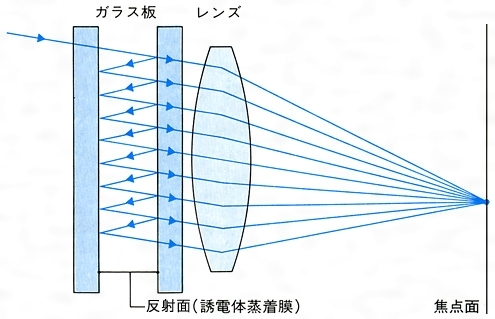
\includegraphics[width=7cm]{fabry.jpg}
				\caption{ファブリ・ペロー干渉計の模式図}
			\end{figure}
		\subsubsection{マッハ・ゼンダ干渉計}
			2分岐したビームが異なった経路を通って,別のハーフミラーで合成され干渉縞を発生させる.
			ミラーによる光路の往復はなく,試料を1度のみ通過する.
			量子もつれの研究等にも用いられている.\cite{mach}
			\begin{figure}[H]
				\centering
				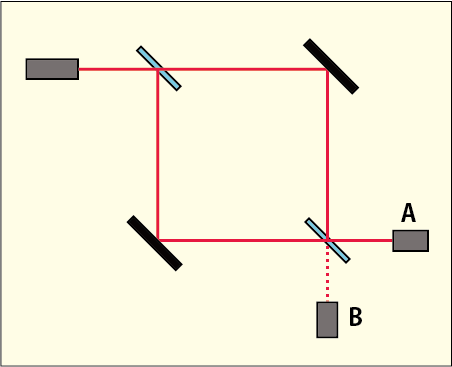
\includegraphics[width=8cm]{mach.png}
				\caption{マッハ・ゼンダ干渉計の模式図}
			\end{figure}
				
\begin{thebibliography}{99}
	\bibitem{lan} LANケーブル - ELECOM,https://www2.elecom.co.jp/cable/lan/index.html,2019年5月9日閲覧
	\bibitem{plc} 高速電力線通信技術「HD-PLC」,https://www.panasonic.com/jp/corporate/technology-design/technology/hd-plc.html,2019年5月9日閲覧
	\bibitem{interference} 干渉計とは,https://www.keyence.co.jp/ss/3dprofiler/keijou/flatness/interferometer/,2019年5月9日閲覧
	\bibitem{fabry} CRLファブリペロー干渉計の開発と熱圏観測 - NICT,http://www.nict.go.jp/publication/shuppan/kihou-journal/kihou-vol48no2/toku0404.pdf,2019年5月9日閲覧
	\bibitem{mach} マッハツェンダー干渉計 - シグマ光機株式会社,https://www.global-optosigma.com/jp/interferometers/ifs2mz25.html,2019年5月9日閲覧
\end{thebibliography}
\end{document}